\documentclass[14pt]{beamer}
\usetheme{Boadilla}
\usepackage{booktabs}
\usepackage{multirow}
\usepackage{enumitem}
\usepackage{tikz}

\newcommand{\E}{\mathbb{E}}
\usefonttheme{professionalfonts}
\usepackage{pgfplots}
\pgfplotsset{compat=1.18}
\renewcommand{\arraystretch}{1.25}
\usetikzlibrary{trees}
\title[ECON2843]{Lecture 24}
\subtitle{Part 5 Linear Regression}
\date{}
\usepackage{amsmath,amssymb,mathtools,wasysym}
\begin{document}
	\begin{frame}
		\titlepage
		
	\end{frame}
	\begin{frame}
		\vspace{1cm}
		\centering
		{\color{blue}\large Multiple Linear Regression}
	\end{frame}
	
	


\begin{frame}
	\frametitle{Multiple Linear Regression}
	
	\begin{itemize}[label={\color{blue}$\blacktriangleright$}]
		\item Multiple linear regression uses a single model to investigate how two or more independent variables, denoted $X_1, X_2, \dots, X_k$, are related to the dependent variable, denoted $Y$.
		
		\item Ideally, we should include as many independent variables into the regression model \textit{as are believed to be related} to the dependent variable.
	\end{itemize}
	
\end{frame}
\begin{frame}
	\frametitle{Advantages}
	
	\begin{itemize}[label={\color{blue}$\blacktriangleright$}]
		\item Can use a \textit{single} model to determine:
		\begin{itemize}[label={\color{blue}$\blacktriangleright$}]
			\item Which independent variables might be truly related to the dependent variable.
			\item The nature of these relationships.
		\end{itemize}
		
		\item Compared to a simple linear regression model, a multiple linear regression model will generally:
		\begin{itemize}[label={\color{blue}$\blacktriangleright$}]
			\item \textit{Fit} the data better.
			\item Produce better \textit{predictions}, provided all the independent variables are truly related to the dependent variable.
		\end{itemize}
	\end{itemize}
	
\end{frame}
\begin{frame}
	\frametitle{Caveats}
	
	\begin{itemize}[label={\color{blue}$\blacktriangleright$}]
		\item We should not include as many independent variables as we can into the regression model.
		
		\item Why?
		\begin{itemize}[label={\color{blue}$\blacktriangleright$}]
			\item \textit{Model selection} is a very important aspect of multiple linear regression.
			
			\item Danger of \textit{over-fitting} our sample data (can degrade predictive performance of model).
			
			\item Problem of \textit{multicollinearity} (parameter estimates become unreliable).
			
			\item We can't fit a multiple linear regression model with more independent variables than observations in our sample.
		\end{itemize}
	\end{itemize}
	
\end{frame}
\begin{frame}
	\frametitle{Multiple Linear Regression Model}
	
	\begin{itemize}[label={\color{blue}$\blacktriangleright$}]
		\item The \textbf{multiple linear regression model} assumes that the relationship between the dependent and independent variables is given by:
		
		\[
		Y = \beta_0 + \beta_1X_1 + \beta_2X_2 + \cdots + \beta_kX_k + \epsilon
		\]
		
		\item $\beta_0$ is the intercept parameter.
		
		\item $\beta_1,\ldots,\beta_k$ are the \textbf{coefficient parameters} for the independent variables.
		
		\item $\epsilon$ is the error variable.
	\end{itemize}
	
\end{frame}
\begin{frame}
	\frametitle{Multiple Linear Regression Model}
	
	\begin{itemize}[label={\color{blue}$\blacktriangleright$}]
		\item The \textbf{multiple linear regression model} assumes that the relationship between the dependent and independent variables is given by:
		

			\[
			Y = \beta_0 + \beta_1X_1 + \beta_2X_2 + \cdots + \beta_kX_k + \epsilon
			\]
		
		\item $\beta_0$ is the intercept parameter.
		
		\item $\beta_1,\ldots,\beta_k$ are the \textbf{coefficient parameters} for the independent variables.
		
		\item $\epsilon$ is the error variable.
	\end{itemize}
	
\end{frame}
\begin{frame}
	\frametitle{Linearity}
	
	\begin{itemize}[label={\color{blue}$\blacktriangleright$}]
		\item The ``linear'' in linear regression refers to linearity in the coefficient parameters.
		
		\item For example, the following is a multiple linear regression model:
		

			\[
			Y = \beta_0 + \beta_1X_1^2 + \beta_2\log X_2 + \beta_3\frac{1}{X_3} + \epsilon
			\]

		
		\item Because we can rewrite the model as:
		

			\[
			Y = \beta_0 + \beta_1W_1 + \beta_2W_2 + \beta_3W_3 + \epsilon
			\]

			where $W_1 = X_1^2$, $W_2 = \log X_2$ and $W_3 = \frac{1}{X_3}$.

	\end{itemize}
	
\end{frame}
\begin{frame}
	\frametitle{Linearity}
	
	\begin{itemize}[label={\color{blue}$\blacktriangleright$}]
		\item However, the following is not a multiple linear regression model:
		\[
		Y = \beta_0 + \beta_1\cos(X_1 + \beta_2) + X_2^{\beta_3} + \epsilon
		\]
		
		\item Scatter plots of $Y$ against each independent variable can help to determine in what form they should appear in the model.
	\end{itemize}
	
\end{frame}
\begin{frame}
	\frametitle{Sample Data}
	
	\begin{itemize}[label={\color{blue}$\blacktriangleright$}]
		\item Our sample data now consists of a set of $k+1$ values for each observation:
		\[
		\{(Y_1, X_{11}, X_{21}, \ldots, X_{k1}),\ldots,(Y_n, X_{1n}, X_{2n},\ldots, X_{kn})\}
		\]
		
		\item The multiple linear regression model states that the $Y_i$ value for the $i$th observation can be expressed as:
		\[
		Y_i = \beta_0 + \beta_1X_{1i} + \beta_2X_{2i} + \cdots + \beta_kX_{ki} + \epsilon_i
		\]
	\end{itemize}
	
\end{frame}
\begin{frame}
	\frametitle{Response Surface}
	
	\begin{itemize}[label={\color{blue}$\blacktriangleright$}]
		\item Rather than a straight line, the multiple linear regression model is a \textit{response surface} described by the following equation:
		\[
		Y = \beta_0 + \beta_1X_1 + \beta_2X_2 + \cdots + \beta_kX_k
		\]
		
		\item Due to inherent variability in the population, observations will not lie \textit{exactly} on the response surface.
		
		\item The error variable $\epsilon_i$ signifies how far the $Y_i$ value for each observation is from the response surface.
	\end{itemize}
	
\end{frame}
\begin{frame}
	\frametitle{Model Assumptions}
	
	\begin{itemize}[label={\color{blue}$\blacktriangleright$}]
		\item We have the same assumptions as we did with simple linear regression, which are again stated in terms of $\epsilon$.
		\item Namely, that the errors:
		\begin{itemize}[label={\color{blue}$\blacktriangleright$}]
			\item Are normally distributed.
			\item Have mean equal to 0.
			\item Have constant variance denoted by $\sigma_\epsilon^2$.
			\item Are independent.
		\end{itemize}
		\item That is, $\epsilon_i \overset{iid}{\sim} N(0,\sigma_\epsilon^2)$.
	\end{itemize}
	
\end{frame}
\begin{frame}
	\frametitle{Multiple Linear Regression Model}
	
	\begin{itemize}[label={\color{blue}$\blacktriangleright$}]
		\item Based on the model assumptions, another way to state the multiple linear regression model is that $Y$ is normally distributed with mean equal to:
		
	
		\[
		E(Y) = \beta_0 + \beta_1X_1 + \beta_2X_2 + \cdots + \beta_kX_k
		\]

		
		and variance equal to:
		
	
		\[
		V(Y) = \sigma_\epsilon^2
		\]
	\end{itemize}
	
\end{frame}
\begin{frame}
	\frametitle{Interpreting the Coefficient Parameters}
	
	\begin{itemize}[label={\color{blue}$\blacktriangleright$}]
		\item Suppose we have the following multiple linear regression model:
		

		\[
		Y = \beta_0 + \beta_1X_1 + \beta_2X_2 + \epsilon
		\]
				
		\item How does the response surface change when we increase the value of $X_1$ by one unit?
		
		\item Consider two observations with $X$ values given by $(x_1, x_2)$ and $(x_1 + 1, x_2)$.
		
	\end{itemize}
	
\end{frame}
\begin{frame}
	\frametitle{Interpreting the Coefficient Parameters}
	
	\begin{itemize}[label={\color{blue}$\blacktriangleright$}]
		\item Original observation $(x_1, x_2)$:
		\[
		E(Y_\text{orig}) = \beta_0 + \beta_1x_1 + \beta_2x_2
		\]
		
		\item New observation $(x_1 + 1, x_2)$:
		\[
		\begin{aligned}
			E(Y_\text{new}) &= \beta_0 + \beta_1(x_1 + 1) + \beta_2x_2 \\
			&= \beta_0 + \beta_1x_1 + \beta_2x_2 + \beta_1 \\
			&= E(Y_\text{orig}) + \beta_1
		\end{aligned}
		\]
		
	\end{itemize}
	
\end{frame}
\begin{frame}
	\frametitle{Interpreting the Coefficient Parameters}
	
	\begin{itemize}[label={\color{blue}$\blacktriangleright$}]
		\item An increase in $X_1$ by one unit leads to a change in the response surface by the amount $\beta_1$.
		
		\item The response surface can equivalently be thought of as the expected value of $Y$, so $\beta_1$ is also the \textit{expected change} in $Y$ when $X_1$ increases by one unit.
		
		\item In general, a coefficient parameter $\beta_j$ represents the expected change in $Y$ when $X_j$ is increased by one unit, with all other independent variables held fixed.
		
	\end{itemize}
	
\end{frame}
\begin{frame}
	\frametitle{Parameter Estimation}
	
	\begin{itemize}[label={\color{blue}$\blacktriangleright$}]
		\item Suppose we have obtained estimates $\hat{\beta}_0$, $\hat{\beta}_1$, \ldots, $\hat{\beta}_k$, for the parameters $\beta_0$, $\beta_1$, \ldots, $\beta_k$.
		
		\item The estimated or \textbf{fitted regression model} is:
		\[
		\hat{Y} = \hat{\beta}_0 + \hat{\beta}_1X_1 + \cdots + \hat{\beta}_kX_k
		\]
		
		\item For each observation in our sample, the \textbf{fitted value} is given by:
		\[
		\hat{Y}_i = \hat{\beta}_0 + \hat{\beta}_1X_{1i} + \cdots + \hat{\beta}_kX_{ki}
		\]
		and the \textbf{residual} is given by:
		\[
		e_i = Y_i - \hat{Y}_i
		\]
		
	\end{itemize}
	
\end{frame}
\begin{frame}
	\frametitle{Method of Least Squares}
	
	\begin{itemize}[label={\color{blue}$\blacktriangleright$}]
		\item Parameter estimates are again chosen as the values that make the residuals as small as possible.
		
		\item That is, the parameters $\beta_0$, $\beta_1$, \ldots, $\beta_k$ are estimated by minimizing the \textbf{sum of squared residuals}:
		\[
		\sum_{i=1}^n e_i^2 = \sum_{i=1}^n \left(Y_i - \hat{Y}_i\right)^2
		\]
		\[
		= \sum_{i=1}^n \left(Y_i - \left(\hat{\beta}_0 + \hat{\beta}_1X_{1i} + \cdots + \hat{\beta}_kX_{ki}\right)\right)^2
		\]
		
	\end{itemize}
	
\end{frame}
\begin{frame}
	\frametitle{Parameter Estimation}
	
	\begin{itemize}[label={\color{blue}$\blacktriangleright$}]
		\item Unlike simple linear regression, we will not be calculating parameter estimates for multiple linear regression by hand.
		
		\item Instead, we will rely on software to fit the model, and the focus will be on \textit{understanding} and \textit{interpreting} the computer output.
		
	\end{itemize}
	
\end{frame}
\begin{frame}
	\frametitle{Attitude Towards the City Example}
	
	\begin{itemize}[label={\color{blue}$\blacktriangleright$}]
		\item Suppose we want to see whether people's attitudes towards the city they live in are linearly related to \textit{two} variables:
		\begin{itemize}[label={\color{blue}$\blacktriangleright$}]
			\item Their duration of residence.
			\item The importance they attach to weather.
		\end{itemize}
		
		\item Last topic, the first step in the analysis was to construct a scatter plot to ``eyeball'' the data.
		
		\item Now that we have two independent variables, we should construct two scatter plots:
		\begin{itemize}[label={\color{blue}$\blacktriangleright$}]
			\item Attitude against duration of residence.
			\item Attitude against importance attached to weather.
		\end{itemize}
		
	\end{itemize}
	
\end{frame}
\begin{frame}
	\frametitle{Attitude against Duration of Residence}
	\centering
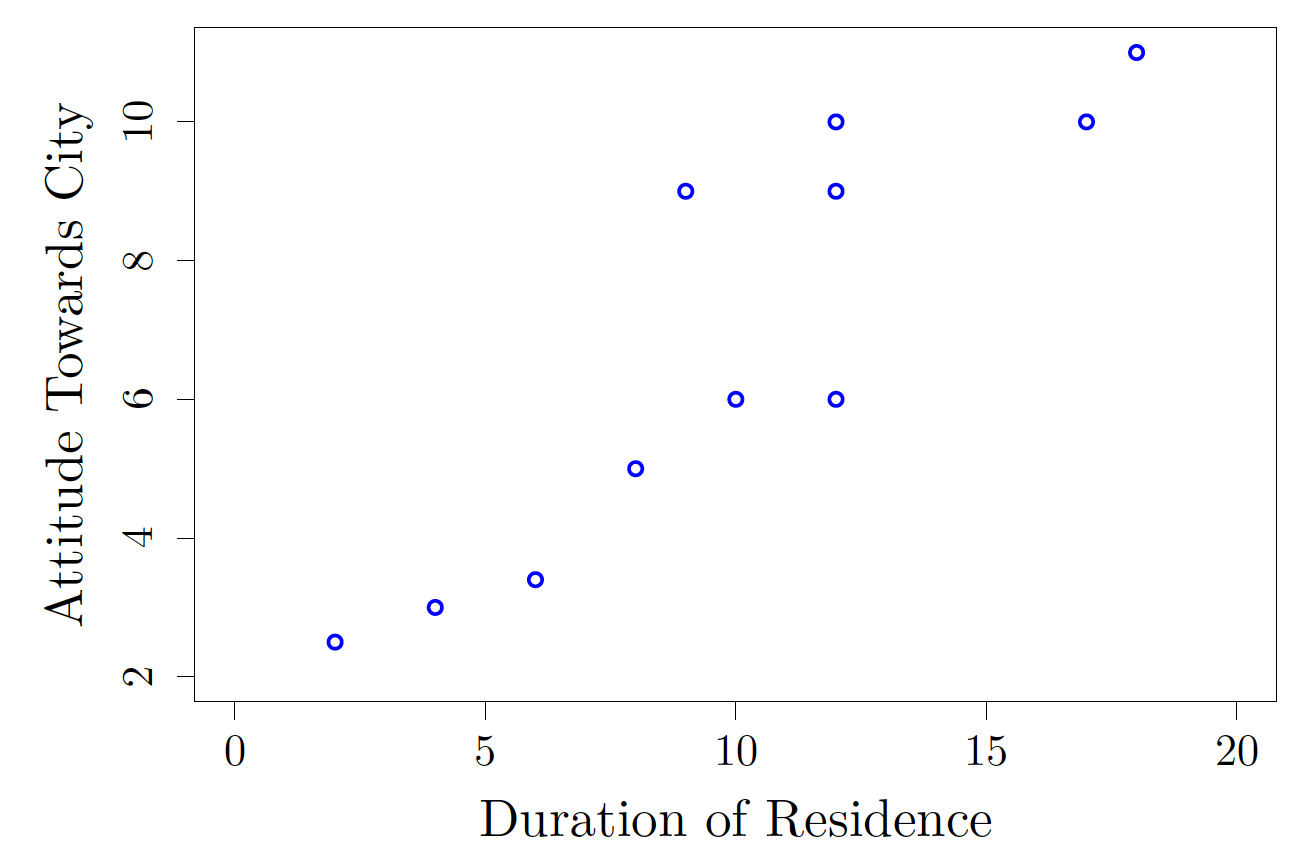
\includegraphics[width=12cm]{attitude.png}
\end{frame}
\begin{frame}
	\frametitle{Attitude against Importance of Weather}
	\centering
	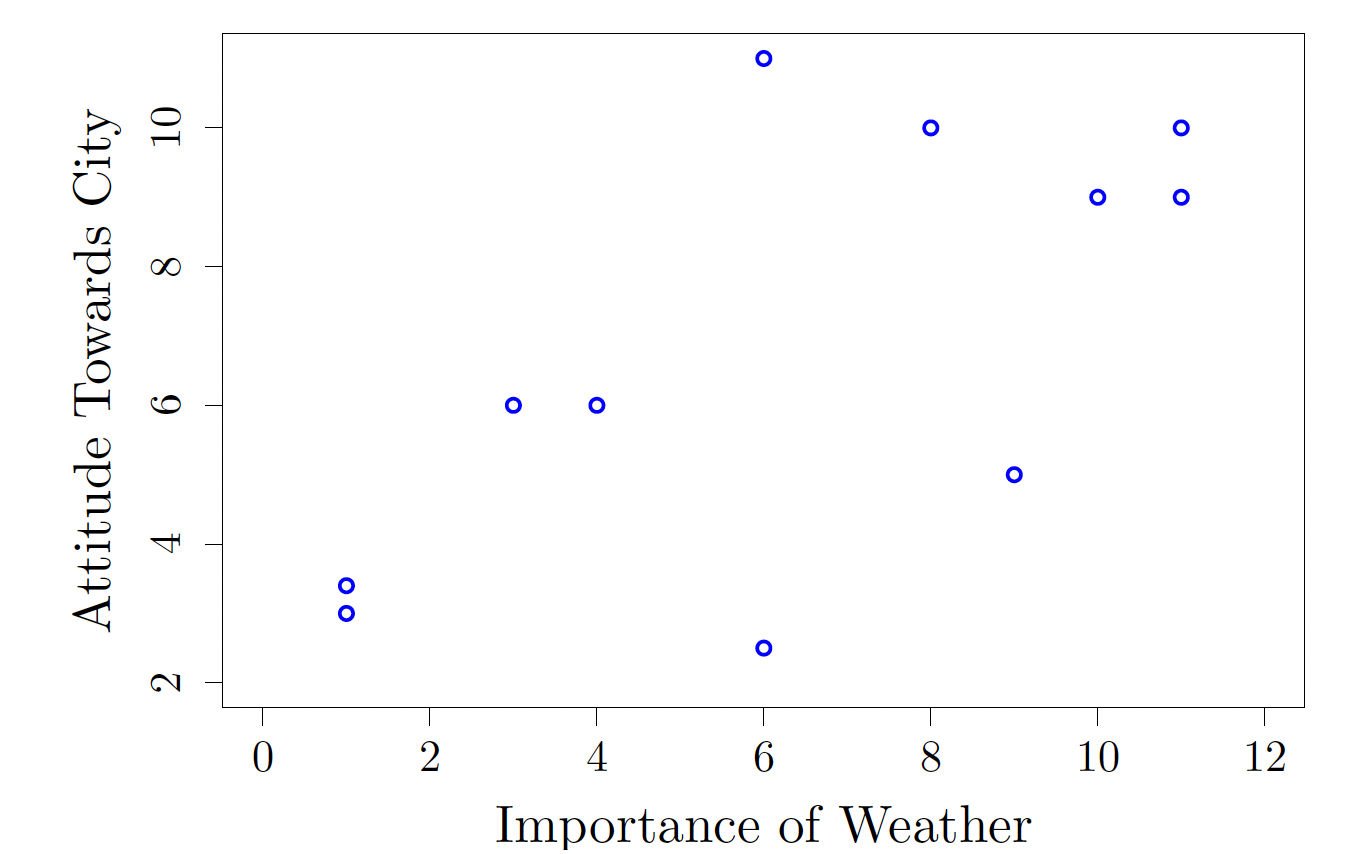
\includegraphics[width=12cm]{weather.png}
\end{frame}
\begin{frame}
	\frametitle{Model Specification}
	
	\begin{itemize}[label={\color{blue}$\blacktriangleright$}]
		\item Next, we need to specify our model.
		
		\item Let $Y$ denote attitude towards the city, $X_1$ denote the duration of residence and $X_2$ denote the importance attached to weather.
		
		\item Since both $X_1$ and $X_2$ appear to be linearly related to $Y$, a reasonable model might be:
		\[
		Y = \beta_0 + \beta_1X_1 + \beta_2X_2 + \epsilon
		\]
		
	\end{itemize}
	
\end{frame}
\begin{frame}[fragile]
	\frametitle{R Output}
	{\footnotesize
	\begin{verbatim}
		Call:
		lm(formula = attitude ~ duration + weather, data = city.dat)
		
		Residuals:
		Min       1Q   Median       3Q      Max 
		-1.56859 -0.79732  0.03449  0.47779  1.82480 
	\end{verbatim}
	{\color{red}
		\begin{verbatim}
			Coefficients:
			Estimate                Std. Error t stat. Pr(>|t|)
			(Intercept)  0.45755    0.94094   0.486  0.639817
			duration     0.46751    0.08907   5.249  0.000775
			weather      0.26344    0.11784   2.236  0.055810
			
			Residual standard error: 1.243 on 8 degrees of freedom
			Multiple R-squared: 0.8724,  Adjusted R-squared: 0.8405
			F-statistic: 27.35 on 2 and 8 DF,  p-value: 0.0002649
		\end{verbatim}
	}}
	
\end{frame}
\end{document}